\documentclass{beamer}

\pdfmapfile{+sansmathaccent.map}


\mode<presentation>
{
	\usetheme{Warsaw} % or try Darmstadt, Madrid, Warsaw, Rochester, CambridgeUS, ...
	\usecolortheme{seahorse} % or try seahorse, beaver, crane, wolverine, ...
	\usefonttheme{serif}  % or try serif, structurebold, ...
	\setbeamertemplate{navigation symbols}{}
	\setbeamertemplate{caption}[numbered]
} 


%%%%%%%%%%%%%%%%%%%%%%%%%%%%
% itemize settings


%%%%%%%%%%%%%%%%%%%%%%%%%%%%
% itemize settings

\definecolor{myhotpink}{RGB}{255, 80, 200}
\definecolor{mywarmpink}{RGB}{255, 60, 160}
\definecolor{mylightpink}{RGB}{255, 80, 200}
\definecolor{mypink}{RGB}{255, 30, 80}
\definecolor{mydarkpink}{RGB}{155, 25, 60}

\definecolor{mypaleblue}{RGB}{240, 240, 255}
\definecolor{mylightblue}{RGB}{120, 150, 255}
\definecolor{myblue}{RGB}{90, 90, 255}
\definecolor{mygblue}{RGB}{70, 110, 240}
\definecolor{mydarkblue}{RGB}{0, 0, 180}
\definecolor{myblackblue}{RGB}{40, 40, 120}

\definecolor{myblackturquoise}{RGB}{5, 53, 60}
\definecolor{mydarkdarkturquoise}{RGB}{8, 93, 110}
\definecolor{mydarkturquoise}{RGB}{28, 143, 150}
\definecolor{mypaleturquoise}{RGB}{230, 255, 255}
\definecolor{myturquoise}{RGB}{48, 213, 200}

\definecolor{mygreen}{RGB}{0, 200, 0}
\definecolor{mydarkgreen}{RGB}{0, 120, 0}
\definecolor{mygreen2}{RGB}{245, 255, 230}

\definecolor{mygrey}{RGB}{120, 120, 120}
\definecolor{mypalegrey}{RGB}{160, 160, 160}
\definecolor{mydarkgrey}{RGB}{80, 80, 160}

\definecolor{mydarkred}{RGB}{160, 30, 30}
\definecolor{mylightred}{RGB}{255, 150, 150}
\definecolor{myred}{RGB}{200, 110, 110}
\definecolor{myblackred}{RGB}{120, 40, 40}

\definecolor{mygreen}{RGB}{0, 200, 0}
\definecolor{mygreen2}{RGB}{205, 255, 200}

\definecolor{mydarkcolor}{RGB}{60, 25, 155}
\definecolor{mylightcolor}{RGB}{130, 180, 250}

\setbeamertemplate{itemize items}[default]

\setbeamertemplate{itemize item}{\color{myblackturquoise}$\blacksquare$}
\setbeamertemplate{itemize subitem}{\color{mydarkdarkturquoise}$\blacktriangleright$}
\setbeamertemplate{itemize subsubitem}{\color{mygray}$\blacksquare$}

\setbeamercolor{palette quaternary}{fg=white,bg=myblackturquoise}
\setbeamercolor{titlelike}{parent=palette quaternary}

\setbeamercolor{palette quaternary2}{fg=black,bg=mypaleblue}
\setbeamercolor{frametitle}{parent=palette quaternary2}

\setbeamerfont{frametitle}{size=\Large,series=\scshape}
\setbeamerfont{framesubtitle}{size=\normalsize,series=\upshape}





%%%%%%%%%%%%%%%%%%%%%%%%%%%%
% block settings

\setbeamercolor{block title}{bg=red!30,fg=black}

\setbeamercolor*{block title example}{bg=mygreen!40!white,fg=black}

\setbeamercolor*{block body example}{fg= black, bg= mygreen2}


%%%%%%%%%%%%%%%%%%%%%%%%%%%%
% URL settings
\hypersetup{
	colorlinks=true,
	linkcolor=blue,
	filecolor=blue,      
	urlcolor=blue,
}

%%%%%%%%%%%%%%%%%%%%%%%%%%

\renewcommand{\familydefault}{\rmdefault}

\usepackage{amsmath}
\usepackage{mathtools}

\usepackage{subcaption}

\usepackage{qrcode}

\DeclareMathOperator*{\argmin}{arg\,min}
\newcommand{\bo}[1] {\mathbf{#1}}

\newcommand{\R}{\mathbb{R}} 
\newcommand{\T}{^\top}     



\newcommand{\mydate}{Fall 2023}

\newcommand{\mygit}{\textcolor{blue}{\href{https://github.com/SergeiSa/Control-Theory-Slides-Spring-2023}{github.com/SergeiSa/Control-Theory-Slides-Spring-2023}}}

\newcommand{\myqr}{ \textcolor{black}{\qrcode[height=1.5in]{https://github.com/SergeiSa/Control-Theory-Slides-Spring-2023}}
}

\newcommand{\myqrframe}{
	\begin{frame}
		\centerline{Lecture slides are available via Github, links are on Moodle}
		\bigskip
		\centerline{You can help improve these slides at:}
		\centerline{\mygit}
		\bigskip
		\myqr
	\end{frame}
}


\newcommand{\bref}[2] {\textcolor{blue}{\href{#1}{#2}}}

%%%%%%%%%%%%%%%%%%%%%%%%%%%%
% code settings

\usepackage{listings}
\usepackage{color}
% \definecolor{mygreen}{rgb}{0,0.6,0}
% \definecolor{mygray}{rgb}{0.5,0.5,0.5}
\definecolor{mymauve}{rgb}{0.58,0,0.82}
\lstset{ 
	backgroundcolor=\color{white},   % choose the background color; you must add \usepackage{color} or \usepackage{xcolor}; should come as last argument
	basicstyle=\footnotesize,        % the size of the fonts that are used for the code
	breakatwhitespace=false,         % sets if automatic breaks should only happen at whitespace
	breaklines=true,                 % sets automatic line breaking
	captionpos=b,                    % sets the caption-position to bottom
	commentstyle=\color{mygreen},    % comment style
	deletekeywords={...},            % if you want to delete keywords from the given language
	escapeinside={\%*}{*)},          % if you want to add LaTeX within your code
	extendedchars=true,              % lets you use non-ASCII characters; for 8-bits encodings only, does not work with UTF-8
	firstnumber=0000,                % start line enumeration with line 0000
	frame=single,	                   % adds a frame around the code
	keepspaces=true,                 % keeps spaces in text, useful for keeping indentation of code (possibly needs columns=flexible)
	keywordstyle=\color{blue},       % keyword style
	language=Octave,                 % the language of the code
	morekeywords={*,...},            % if you want to add more keywords to the set
	numbers=left,                    % where to put the line-numbers; possible values are (none, left, right)
	numbersep=5pt,                   % how far the line-numbers are from the code
	numberstyle=\tiny\color{mygray}, % the style that is used for the line-numbers
	rulecolor=\color{black},         % if not set, the frame-color may be changed on line-breaks within not-black text (e.g. comments (green here))
	showspaces=false,                % show spaces everywhere adding particular underscores; it overrides 'showstringspaces'
	showstringspaces=false,          % underline spaces within strings only
	showtabs=false,                  % show tabs within strings adding particular underscores
	stepnumber=2,                    % the step between two line-numbers. If it's 1, each line will be numbered
	stringstyle=\color{mymauve},     % string literal style
	tabsize=2,	                   % sets default tabsize to 2 spaces
	title=\lstname                   % show the filename of files included with \lstinputlisting; also try caption instead of title
}


%%%%%%%%%%%%%%%%%%%%%%%%%%%%
% URL settings
\hypersetup{
	colorlinks=false,
	linkcolor=blue,
	filecolor=blue,      
	urlcolor=blue,
}

%%%%%%%%%%%%%%%%%%%%%%%%%%

%%%%%%%%%%%%%%%%%%%%%%%%%%%%
% tikz settings

\usepackage{tikz}
\tikzset{every picture/.style={line width=0.75pt}}


\title{New Actuators Types}
\subtitle{Mechatronics, Lecture 12}
\author{by Sergei Savin}
\centering
\date{\mydate}



\begin{document}
\maketitle



\begin{frame}{Content}
\begin{itemize}
	\item Variable Stiffness Actuators
	\item Twisted Spring Actuators
	\item Tensegrity structures
\end{itemize}
\end{frame}



\begin{frame}
	\centerline{Variable Stiffness Actuators}
\end{frame}

\begin{frame}{Variable Stiffness Actuator}
	\begin{flushleft}
		
		% TODO: \usepackage{graphicx} required
		\begin{figure}
			\centering
			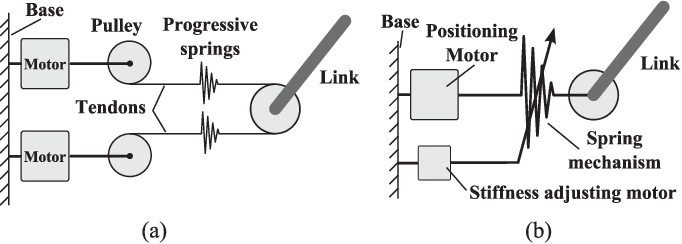
\includegraphics[width=1.0\linewidth]{VSA_1}
			\caption{Wolf, Sebastian, et al. "Variable stiffness actuators: Review on design and components." IEEE/ASME transactions on mechatronics 21.5 (2015): 2418-2430.}
			\label{fig:vsa1}
		\end{figure}
		
		
	\end{flushleft}
\end{frame}



\begin{frame}{Variable Stiffness Actuator - model, 1}
	\begin{flushleft}
		
		Different types of Variable Stiffness Actuators (VSA) have different models. Qbmove actuator is described by the following one:
		
	\begin{equation}
		\begin{cases}
			L_1 \dot I_1 + R_1 I_1 + C_{w,1} \dot \theta_1 = u_1 
			\\
			L_2 \dot I_2 + R_2 I_2 + C_{w,2} \dot \theta_2 = u_2
			 \\
			J_1 \ddot \theta_1 + \mu_1 \dot \theta_1 = C_{\tau, 1} I_1 - \tau_1
			 \\
			J_2 \ddot \theta_2 + \mu_2 \dot \theta_2 = C_{\tau, 2} I_2 - \tau_2 
			\\
			J \ddot \varphi + \mu \dot \varphi = \tau_1 + \tau_2
		\end{cases}
	\end{equation}
%
where $\theta_1$, $\theta_2$  - orientation of the internal motor shaft, and $\varphi$ - orientation of the output shaft, $\tau_1$, $\tau_2$ - torque produced by elastic elements, $J$, $J_1$, $J_2$ - moment of inertia, $\mu$, $\mu_1$, $\mu_2$ - viscous friction coefficient, 
$L$, $R$, $C_w$, $C_\tau$, $I$, $u$ are inductance, resistance, back-EMF and torque coefficients, current and input voltage.
		
		
	\end{flushleft}
\end{frame}






\begin{frame}{Variable Stiffness Actuator - model, 2}
	\begin{flushleft}
		
		The torque produced by elastic elements for Qbmove is given as:
		
		\begin{align}
			\tau_1 = \sigma \sinh (a_1 (\theta_1 - \varphi)) 
			\\
			\tau_2 = \sigma \sinh (a_2 (\theta_2 - \varphi)) 
		\end{align}
		%
		where $a_1$ and $\sigma$ are model constants.
		
		\bigskip
		
		The non-linearity of this model allows us to control the stiffness of the VSA.
		
	\end{flushleft}
\end{frame}



\begin{frame}{Variable Stiffness Actuator - model, 3}
	\begin{flushleft}
		
		Stiffness $\mathcal{K}$ of an actuator can be defined as a partial derivative of the output torque with respect to the output shaft orientation:
		
		\begin{equation}
			\mathcal{K} = \frac{\partial (\tau_1 + \tau_2)}{\partial \varphi}
		\end{equation}
		
		Note that if the torque was linear or affine with respect to $\varphi$, then stiffness of such actuator could not be influenced by internal variables $\theta_i$ or the orientation of the output shaft $\varphi$.
		
		
		
	\end{flushleft}
\end{frame}


\begin{frame}
	\centerline{Twisted Spring Actuators}
\end{frame}


\begin{frame}{Twisted Spring Actuator, 1}
	\begin{flushleft}
		
		% TODO: \usepackage{graphicx} required
		\begin{figure}
			\centering
			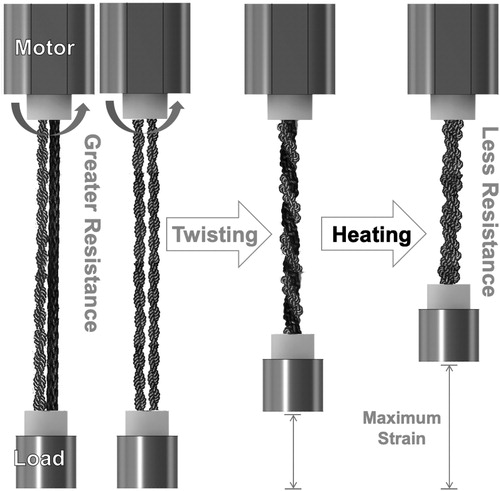
\includegraphics[width=0.7\linewidth]{TSA}
%			\caption{}
			\label{fig:tsa}
		\end{figure}
		
%		Bombara, D., Fowzer, S. and Zhang, J., 2022. Compliant, large-strain, and self-sensing twisted string actuators. Soft Robotics, 9(1), pp.72-88.
		
	\end{flushleft}
\end{frame}



\begin{frame}{Twisted Spring Actuator, 2}
	\begin{flushleft}
		
		% TODO: \usepackage{graphicx} required
		\begin{figure}
			\centering
			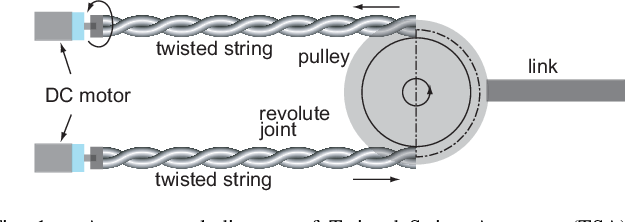
\includegraphics[width=1\linewidth]{TSA_2}
			\caption{Inoue, T., Miyata, R. and Hirai, S., 2016, October. Force control on antagonistic twist-drive actuator robot. In 2016 IEEE/RSJ International Conference on Intelligent Robots and Systems (IROS) (pp. 3830-3835). IEEE.}
			\label{fig:tsa2}
		\end{figure}
		
		
		%		Inoue, T., Miyata, R. and Hirai, S., 2016, October. Force control on antagonistic twist-drive actuator robot. In 2016 IEEE/RSJ International Conference on Intelligent Robots and Systems (IROS) (pp. 3830-3835). IEEE.
		
	\end{flushleft}
\end{frame}



\begin{frame}
	\centerline{Tensegrity structures}
\end{frame}



\begin{frame}{Tensegrity structures}
	\begin{flushleft}
		
		% TODO: \usepackage{graphicx} required
		\begin{figure}
			\centering
			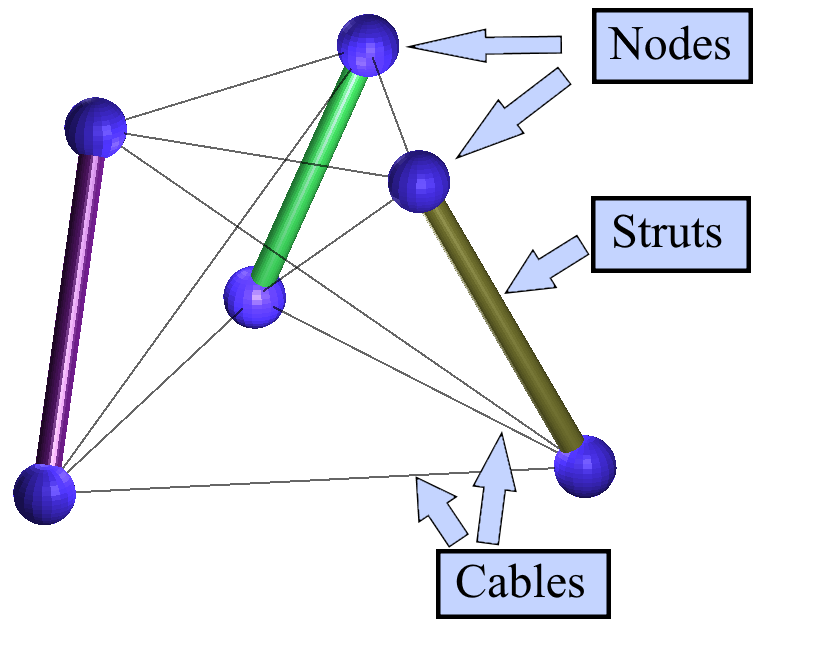
\includegraphics[width=0.7\linewidth]{tensegrity_1}
			\label{fig:tensegrity1}
		\end{figure}
		
		Note that cables are usually elastic and pre-stressed.
		
	\end{flushleft}
\end{frame}



\begin{frame}{Tensegrity forses}
	\begin{flushleft}
		
		Elastic force acting between nodes $\bo{r}_i$ and $\bo{r}_j$ can be modelled as follows:
		
		\begin{equation}
			\label{eq:elastice_force_vanilla}
			\bo{f}_{ij} = \mu_{ij} (||\bo{r}_i - \bo{r}_j|| - \rho_{ij}) \frac{\bo{r}_i - \bo{r}_j}{||\bo{r}_i - \bo{r}_j||}
		\end{equation}
		%
		where $\mu_{ij}$ - cable stiffness, $ \rho_{ij}$ - undeformed cable length
	
		
	\end{flushleft}
\end{frame}




\begin{frame}{Tensegrity robot}
	\begin{flushleft}
		
		% TODO: \usepackage{graphicx} required
		\begin{figure}
			\centering
			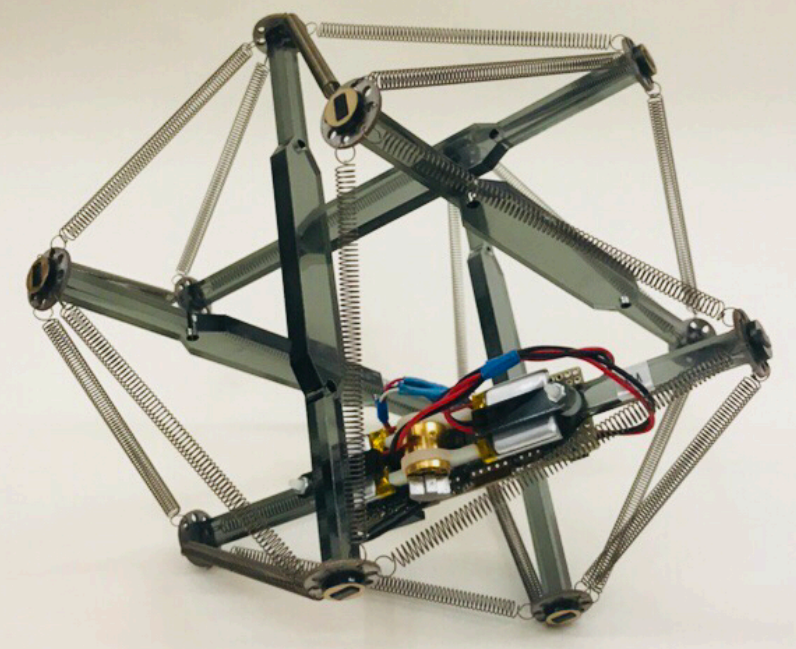
\includegraphics[width=0.7\linewidth]{tensegrity_2}
			\caption{		Rieffel, J. and Mouret, J.B., 2018. Adaptive and resilient soft tensegrity robots. Soft robotics, 5(3), pp.318-329.}
			\label{fig:tensegrity1}
		\end{figure}
		

	\end{flushleft}
\end{frame}

\myqrframe

\end{document}
